\chapter{Introduction}
\label{chap:intro}
\section{What are fractals?}
In what follows we will be investigating fractals and some of their interesting
properties. First we define a fractal.

\begin{dfn}
  A {\bf fractal}\index{fractal} is a curve or geometric figure, each part of
  which has the same statistical character as the whole.
\end{dfn}

\begin{wrapfigure}{r}{0.35\textwidth}
  \centering
  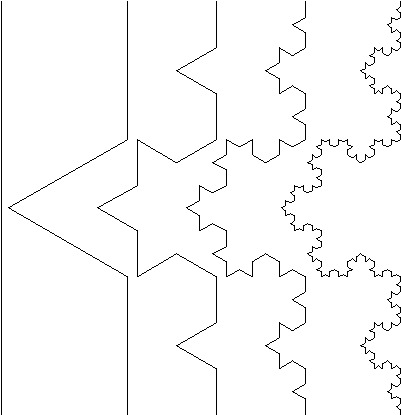
\includegraphics[width=0.33\textwidth]{img/bk_introkochgen}
  \caption{The first few iterations in generating the Koch Curve}
  \label{fig:intro koch}
\end{wrapfigure}
What this means in layterms is that a fractal is a shape or set that has
similar properties at all magnifications. A classic example is the {\em Koch
Curve} (Fig \ref{fig:intro koch}) which looks identical at all levels of
magnification. We should note that there are certain degenerate cases which
satisfy our definition such as a straight line. The distinction between a
true fractal and a degenerate case can be made with the notion of {\em fractal
dimension} which we will touch upon in Chapter \ref{chap:measure} which deals
with measure theory.\\

\section{Fractal Generation}
\label{sec:fractal generation}
It is often useful to think of a fractal as a set of points. However it is
often difficult to explicitly state which points are in our fractal. A standard
technique for fractal generation is to describe the {\em generation} of a 
fractal {\em iteratively} or {\em corecursively}. Typically we start with a
base case, usually a set \(A_0\), and define some sort of operation \(\varphi\)
on a set and define \(A_{i+1} = \phi(A_i)\) for \(i \in \Z^+\). In
Fig \ref{fig:intro koch} we see that our base case is a straight line and our
operation \(\varphi\) replaces the middle third of each line segment in \(A_i\)
with two line segments forming the top part of a triangle.\\

We then say that the 

